\section{UI/UX Design}
The application has a streamlined user interface with a single window navigating between different views to ensure an intuitive and user-friendly experience. Below is the flow of UI/UX interactions. Some parts of the interface were designed and implemented during the first semester. In the second semester, we expanded the system by integrating object tracking and annotation.

In addition to these modifications, button visuals were revised to provide a more professional appearance. (Figures \ref{fig:button_before} and \ref{fig:button_after} show the button appearance before and after the updates.)

\begin{figure}[h!]
    \centering
    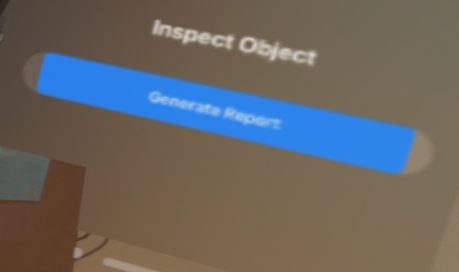
\includegraphics[width=0.4\textwidth]{button_before.png}
    \caption{\centering Button appearance before visual update.}
    \label{fig:button_before}
\end{figure}

\begin{figure}[h!]
    \centering
    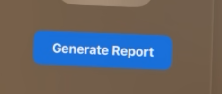
\includegraphics[width=0.4\textwidth]{button_after.png}
    \caption{\centering Button appearance after visual update.}
    \label{fig:button_after}
\end{figure}

\subsection{Initial Session Start}
The application starts with a view prompting the user to begin an ARKit session. In the first semester, this session was primarily responsible for initializing plane detection and world tracking. In the current version, it also starts object tracking for all referenced objects. The interface provides visual indicators to guide the user during this setup phase. (Figure \ref{fig:ui_session_start} shows the UI at this stage.)
\begin{figure}[H]
    \centering
    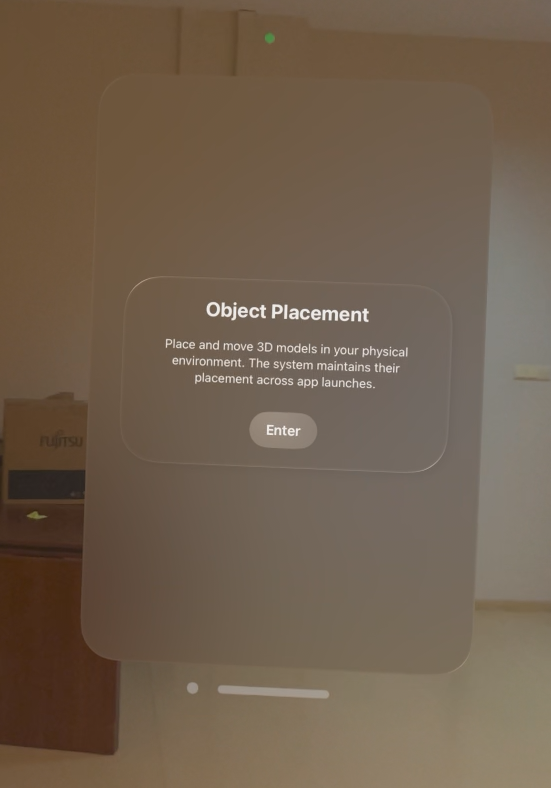
\includegraphics[width=0.37\textwidth]{session_start_ui.png} % Replace with your image file name
    \caption{UI for starting the ARKit session.}
    \label{fig:ui_session_start}
\end{figure}

\subsection{Object Selection Menu}
After initializing the session, the user is directed to an object selection menu. In this view:
\begin{itemize}
    \item The user selects an object from the available options.
    \item When an object is clicked, the \texttt{selectedObject} state is updated.
    \item The selected object is prepared for placement. (Figure \ref{fig:ui_object_selection} shows the object selection menu.)
\end{itemize}

While the basic selection mechanism was implemented in the first semester, this semester we expanded the menu by adding new models specifically designed to demonstrate the object tracking feature. Each of these new models is associated with a reference object file used for object recognition, along with a corresponding USDZ format 3D model for rendering in AR.

\begin{figure}[h!]
    \centering
    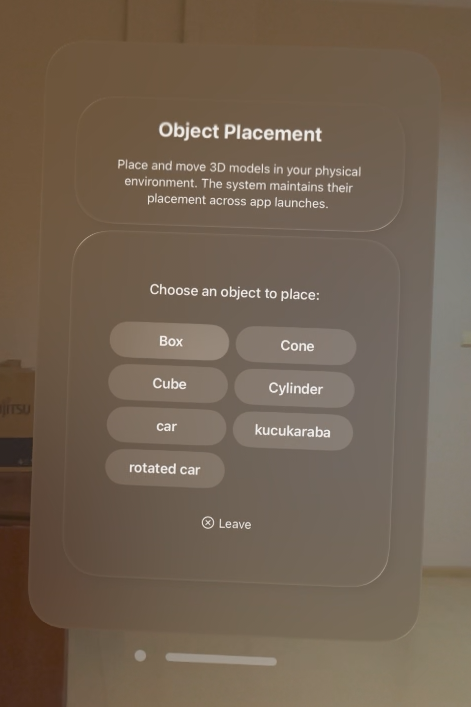
\includegraphics[width=0.4\textwidth]{object_selection_ui.png} % Replace with your image file
    \caption{Object selection menu UI.}
    \label{fig:ui_object_selection}
\end{figure}

\subsection{Initial Object Placement}
This component was implemented during the first semester and remains unchanged in the current version. During the initial placement of the selected object:
\begin{itemize}
    \item Placement tooltips are displayed to guide the user on positioning the object accurately.
    \item Visual aids ensure the user understands how to interact with the AR environment. (Figure \ref{fig:ui_initial_placement} shows the placement tooltip.)
\end{itemize}
\begin{figure}[H]
    \centering
    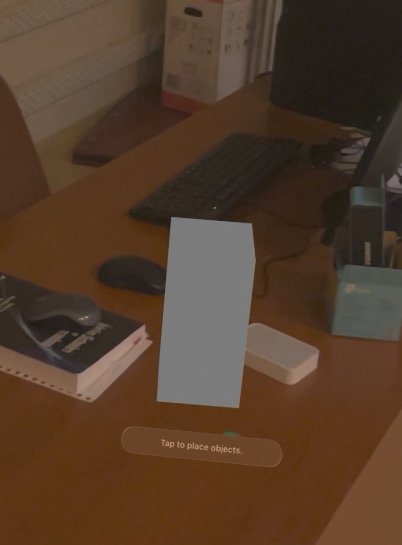
\includegraphics[width=0.4\textwidth]{object_placement_tooltips.png} % Replace with your image file
    \caption{Placement tooltips during initial object placement.}
    \label{fig:ui_initial_placement}
\end{figure}

\subsection{Object Interaction View}
If there is already a placed object, the application navigates directly to the object interaction view. This view was initially developed in the first semester to support repositioning, inspection, and removal of the placed object. In the second semester, this view was extended with additional functionality, including a new annotation interaction feature and the relocation of the \textit{Generate Report} button.

\begin{itemize}
    \item The user can perform repositioning, inspection, annotation, report generation, or removal of the placed object. The interface displays buttons for these actions, as shown in Figure \ref{fig:object_interaction_view}.
\end{itemize}

\begin{figure}[H]
    \centering
    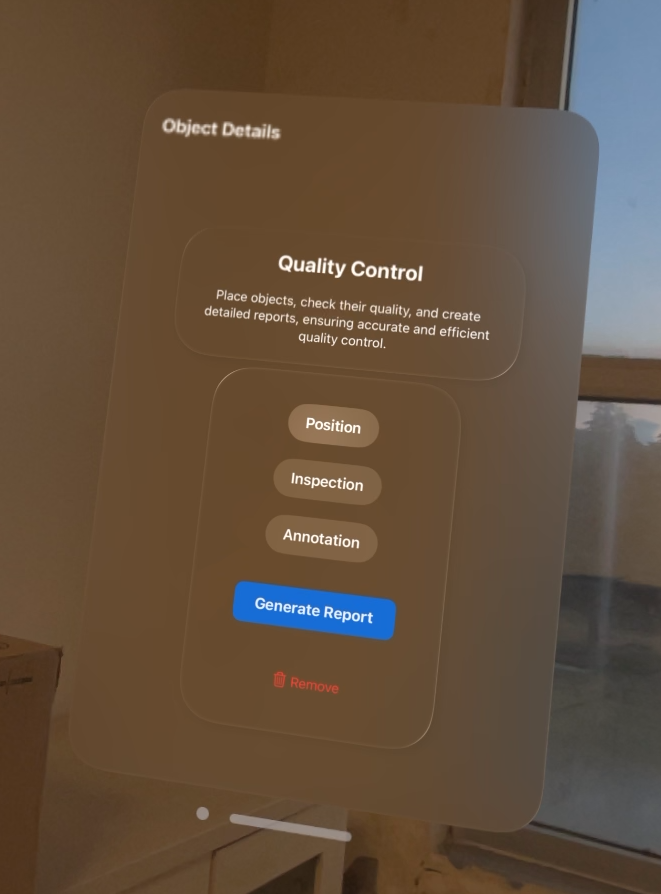
\includegraphics[width=0.39\textwidth]{object_interaction_view.png}
    \caption{\centering UI showing the buttons for repositioning, inspection, annotation, report generation, and removal.}
    \label{fig:object_interaction_view}
\end{figure}


\begin{itemize}
    \item Action buttons allow the user to activate the following functionalities:
    \begin{itemize}

        \item \textbf{Repositioning:} Includes rotation, left/right movement, and forward/backward movement. The user can use pinch and drag gestures (thumb and index finger) to perform the action. Only one action can be performed at a time.

        In addition to these basic controls, we introduced new buttons in the second semester to support object tracking visualization:
        \begin{itemize}
            \item \textbf{Snap Button:} Allows the user to align the placed model with the most recent object tracking data.
            \item \textbf{Object Tracking Mode Toggle:} Enables a continuous tracking mode where the model automatically updates its position and orientation according to real-time object tracking data.
        \end{itemize}

        These buttons are only visible when the selected model includes a valid reference object file and when the corresponding real-world object is detected in the environment.

        (Figure \ref{fig:ui_repositioning} shows the repositioning process and interaction layout.)
        \begin{figure}[H]
            \centering
            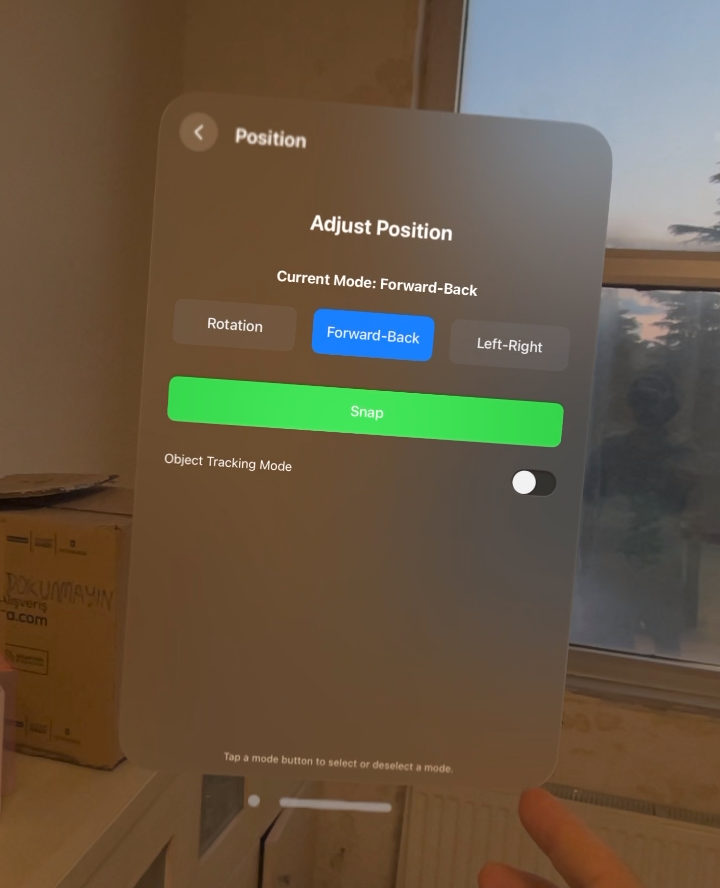
\includegraphics[width=0.47\textwidth]{repositioning_ui_new.png}
            \caption{\centering Repositioning view showing gesture-based controls and the newly added Snap and Tracking Mode buttons}
            \label{fig:ui_repositioning}
        \end{figure}


        \item \textbf{Inspection:} Inspection points are UI buttons attached to the placed object. These points activate only in the inspection view. Previously, this view included the \textit{Generate Report} button; however, in the current version, the button has been relocated to the main interaction view. (Figure \ref{fig:ui_inspection_view} shows the inspection view.)
        \begin{figure}[H]
            \centering
            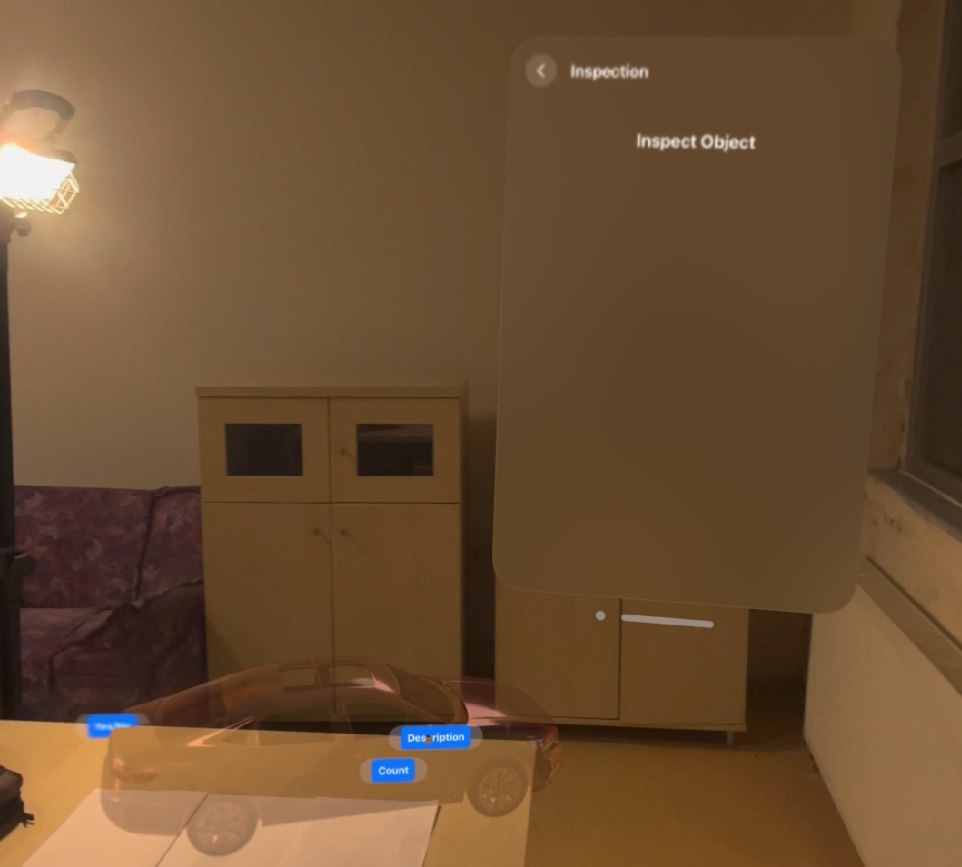
\includegraphics[width=0.6\textwidth]{inspection_view_ui.png}
            \caption{Inspection view showing active inspection points.}
            \label{fig:ui_inspection_view}
        \end{figure}

        \item \textbf{Annotation:} Introduced in the second semester, this feature allows the user to attach custom annotations directly onto the surface of the placed object. The user can tap on any point to create an annotation and enter relevant text. A search functionality is also included, enabling users to filter and locate annotations efficiently.

        \begin{figure}[H]
            \centering
            \begin{minipage}[t]{0.48\textwidth}
                \centering
                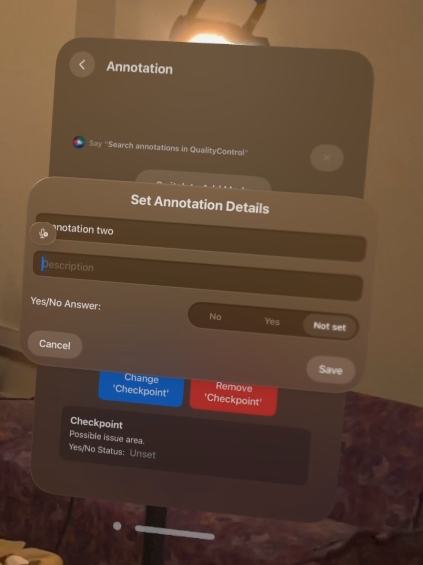
\includegraphics[width=\linewidth]{create_annotation.png}
                \caption{User creating an annotation on the object surface.}
                \label{fig:create_annotation}
            \end{minipage}
            \hfill
            \begin{minipage}[t]{0.48\textwidth}
                \centering
                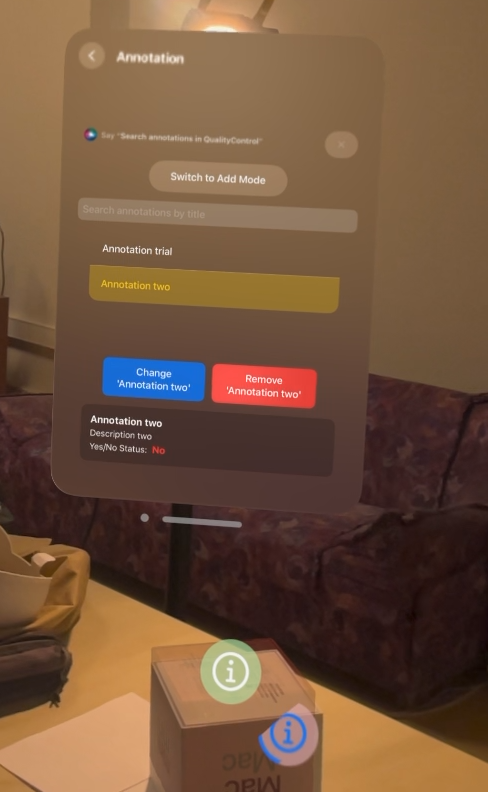
\includegraphics[width=\linewidth]{annotation_view.png}
                \caption{Annotation view showing the list of annotations attached to the object.}
                \label{fig:annotation_view}
            \end{minipage}
        \end{figure}



        \item \textbf{Generate Report:} Now placed directly within the object interaction view, this button triggers report generation without navigating away from the current screen. Upon activation, a confirmation message appears, indicating the report has been successfully generated. (Figure \ref{fig:generate_report_view} shows the confirmation message that appears after report generation.)
        \begin{figure}[H]
            \centering
            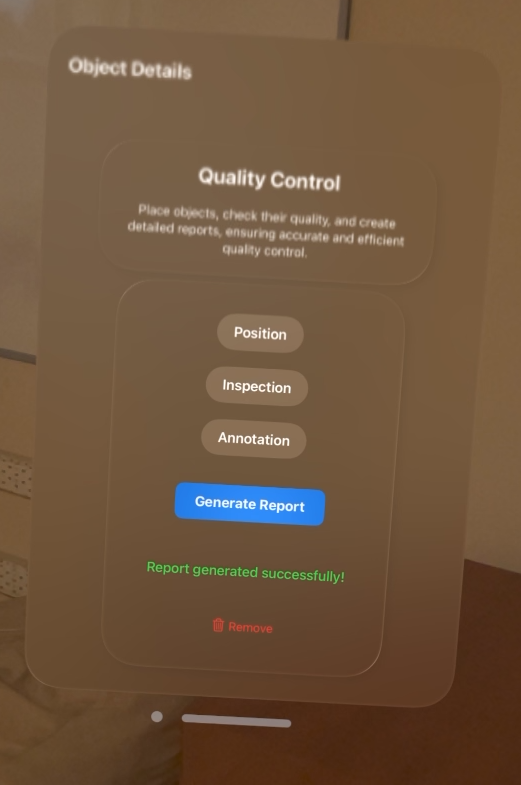
\includegraphics[width=0.4\textwidth]{generate_report_view.png}
            \caption{\centering Confirmation message indicating successful report generation.}
            \label{fig:generate_report_view}
        \end{figure}


        \item \textbf{Removal:} To remove the placed object, the user presses the remove button. A confirmation popup appears to ensure the action is intentional. (Figure \ref{fig:ui_remove_popup} shows the removal confirmation popup.)
        \begin{figure}[H]
            \centering
            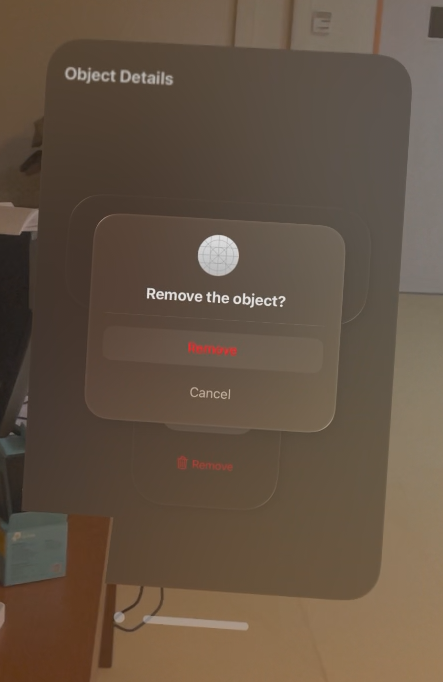
\includegraphics[width=0.4\textwidth]{remove_popup_ui.png}
            \caption{Confirmation popup for removing the placed object.}
            \label{fig:ui_remove_popup}
        \end{figure}
    \end{itemize}
\end{itemize}

\subsection{Inspection Detail View}
This component was fully implemented during the first semester and remains unchanged in the current version of the application. When an inspection point is clicked, the application navigates to the inspection detail view:
\begin{itemize}
    \item A question specific to the inspection point is displayed, which can be one of the following:
    \begin{itemize}
        \item Yes/No question.
        \item Count input.
        \item Description input.
    \end{itemize}
    \item The user provides the required input or feedback. (Figure \ref{fig:ui_inspection_detail} shows the inspection detail view.)
\end{itemize}


\begin{figure}[H]
    \centering
    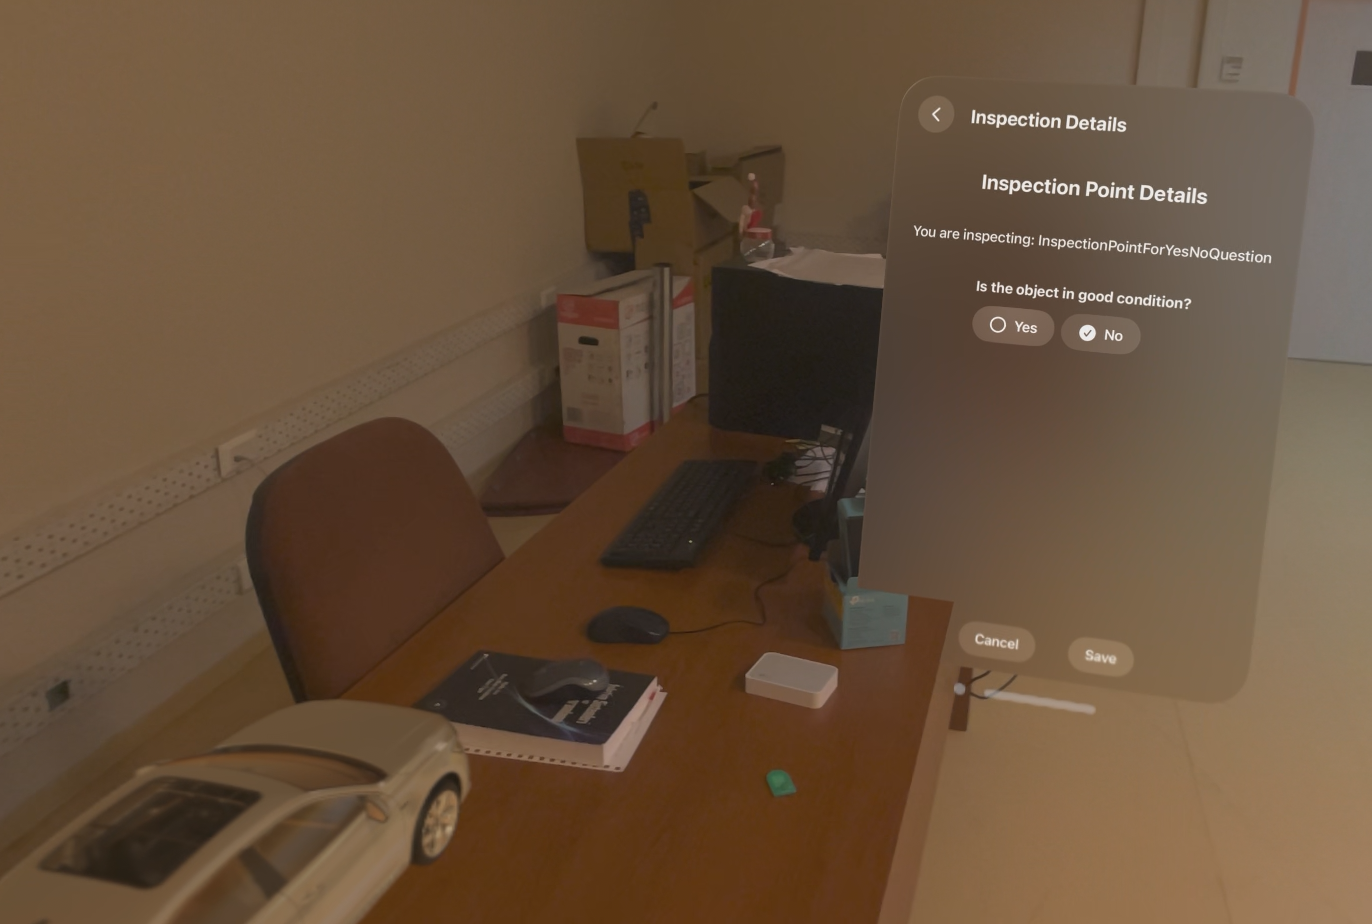
\includegraphics[width=0.8\textwidth]{inspection_detail_ui.png} % Replace with your actual file name
    \caption{Inspection detail view showing specific question types and input fields.}
    \label{fig:ui_inspection_detail}
\end{figure}

\subsection{Annotation Views}

In the second semester, an annotation system was introduced. This system uses visually responsive annotation cards that are spatially anchored to the 3D model and provide intuitive user interaction mechanisms.

\subsubsection{Annotation Card Design and Behavior}

Each annotation is represented by a UI card that is attached to a specific point on the 3D model. These cards remain anchored in space and are always oriented toward the user for readability. When the user gazes at a card, it activates a hover effect that expands the card to display more detailed information.

The expanded annotation card includes:
\begin{itemize}
    \item A \textbf{title} and \textbf{description} section.
    \item A \textbf{Yes/No} selection interface.
    
    The Yes/No state is visually encoded:
    \begin{itemize}
        \item \textbf{Green} for "Yes"
        \item \textbf{Red} for "No"
    \end{itemize}
\end{itemize}

\begin{figure}[H]
            \centering
            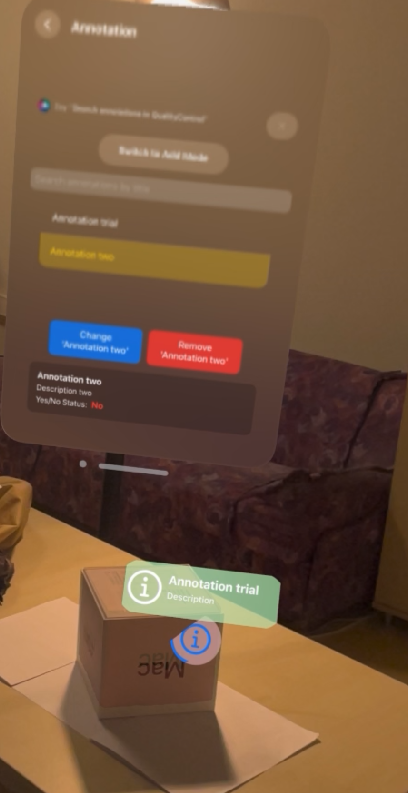
\includegraphics[width=0.4\textwidth]{annotation_card_design.png}
            \caption{Hovering annotation card design showing title, description, and Yes/No state.}
            \label{fig:annotation_card_design}
        \end{figure}

\subsubsection{Focused Annotation Mode}

There are multiple ways to activate this mode:
\begin{itemize}
    \item \textbf{Direct Focus:} The user can look at an annotation card in the AR scene and perform a pinch gesture to enter focused mode.
    \item \textbf{Menu-Based Activation:} Users can slide through a list of annotations displayed in the side menu. By looking at a list item and performing a pinch gesture, the corresponding annotation is automatically focused in the 3D view.
    \item \textbf{Search-Based Activation:} Users can search for an annotation using a built-in search bar. After locating the desired item, the user can look at it in the list and pinch to activate the focused annotation in the AR scene.
    \item \textbf{Siri Voice Search:} Users can also initiate a search by speaking to Siri. Siri automatically fills the search bar and highlights matching results in the list for pinch-based selection.
\end{itemize}

\begin{figure}[H]
            \centering
            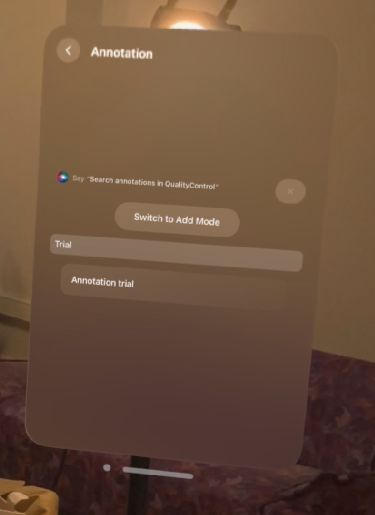
\includegraphics[width=0.4\textwidth]{annotation_search.png}
            \caption{\centering Search bar and list of annotations in the side menu. Users can search for annotations and select them to focus in the AR scene.}
            \label{fig:annotation_search}
        \end{figure}

When an annotation is focused, its card and the side menu visually changes to indicate the active state:
\begin{itemize}
    \item The annotation card turns \textbf{blue}, visually distinguishing it from other annotations in the scene.
    \item The user can then \textbf{edit} the annotation (e.g., update its title, description, or Yes/No state).
    \item The user also has the option to \textbf{remove} the focused annotation from the scene if it is no longer needed.
\end{itemize}

\begin{figure}[H]
            \centering
            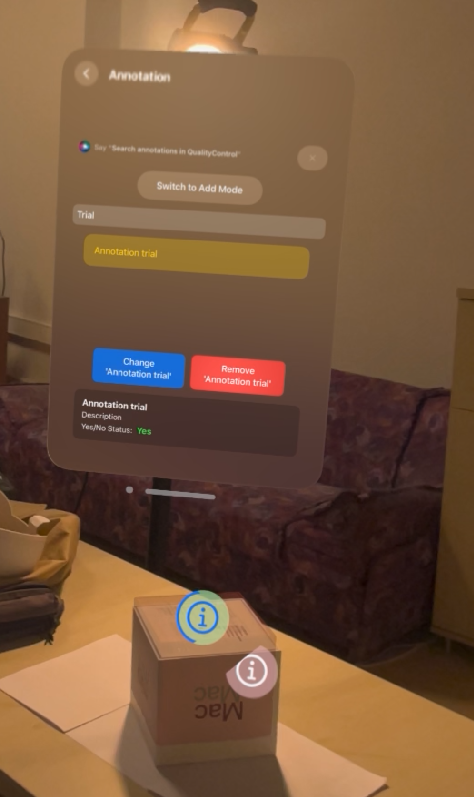
\includegraphics[width=0.4\textwidth]{annotation_focus.png}
            \caption{\centering Focused annotation card in the AR scene, showing the active state with a blue color. The user can edit or remove the annotation.}
            \label{fig:annotation_focus}
        \end{figure}


